\documentclass[a4paper]{book}

%% Language and font encodings
\usepackage[T1,T8K,T8M]{fontenc}
\usepackage[utf8]{inputenc}
\usepackage[english,georgian]{babel}

%% Sets page size and margins
\usepackage[a4paper,top=3cm,bottom=2cm,left=3cm,right=3cm,marginparwidth=1.75cm]{geometry}

%% Useful packages
\usepackage{amsmath}
\usepackage{graphicx}
\usepackage[colorinlistoftodos]{todonotes}
\usepackage[colorlinks = true, allcolors = blue]{hyperref}
\usepackage{float}
\usepackage{enumerate}
\usepackage{subfig}
\usepackage{gensymb}

\title{ფიზიკა}
\author{ლევან კანკაძე}

\begin{document}
\maketitle

\tableofcontents

\chapter{წინასიტყვაობა.}
აქ არის მოგროვებული სხვადასხვა მასალები ფიზიკაში.


\chapter{მექანიკა}
\section{4 ვექტორი}
%Griffiths, David J. - Introduction to Elementary Particles [2nd Edition]

\section{რეაქტიული მოძრაობა}

\section{სტატიკა} სტატიკაში შეისწავლება მყარი სხეულების წონასწორობა, რომელზეც მოქმედებს ძალები. წონასწორობაში იგულისხმება მდგომარეობა, რომლისთვისაც, სხეულს არ გააჩნია აჩქარება, ანუ მოძრაობს თანაბრად და წრფივად, ან ნაწილობრივ, იმყოფება უძრავად ათვლის ინერციულ სისტემაში. (პრაქტიკულად ამოცანებში, დედამიწასთან დაკავშირებული ათვლის სისტემა ითვლება ინერციულად).

განვიხილოთ თუ რა ძალები მოქმედებს წონასწორობაში მყოფ სხეულზე. პირველ რიგში უნდა გავიხსენოთ სიმძიმის ძალა. ეს სიმძიმის ძალა არის ტოლქმედი სხეულის შემადგენელი ნაწილაკების სიმძიმის ძალისა. სიმძიმის ძალა გადის სხეულის მასათა ცენტრზე. 
	
შემდეგ მოქმედებს ბმის რეაქციის ძალები - ეს ძალები ეწინააღმდეგება სხეულის მოძრაობას რომელიმე მიმართულებით. ბმის რეაქციის ძალა მიმართულია იმ მიმართულების საწინააღმდეგოდ, რომელი მიმართულებითაც ბმა ეწინააღმდეგება სხეულის მოძრაობას. რეაქციის ძალებია - დრეკადობისა და ხახუნის ძალები. მათი მოდულები და ზოგჯერ მიმართულება წინასწარ არაა ცნობილი და დამოკიდებულია, სხეულის ფორმაზე, ზედაპირების მდგომარეობაზე, ასევე სხეულზე მოქმედ სხვა ძალებზე.
	
რეაქციის ძალის მიმართულების განსაზღვრა აუცილებელია სტატიკის ამოცანების სწორად ამოსახსნელად.	

ამიტომაც განვიხილოთ როგორაა მიმართული რამდენიმე სახის ბმის რეაქციის ძალები:
	
1. 
	
2. გადაბმა არის დრეკადი ძაფით, მაშინ დრეკადობის ძალა არის ყოველთვის მიმართული ძაფის გასწვრივ და "გამოდის" იმ წერტილიდან რომლითაც მიმაგრებულია სხეულზე.
		\begin{figure}[H]
	 	\centering
           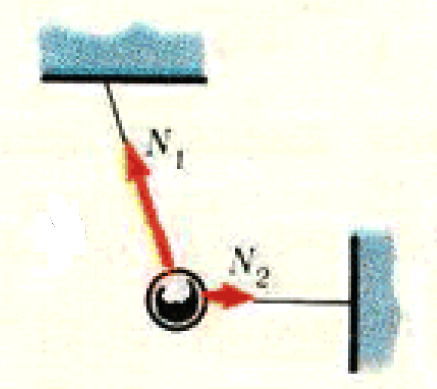
\includegraphics[width=0.2\columnwidth]{figures/static_c}
           \caption{A boat.}
           \label{fig:static_c}
        \end{figure}
	 
	 3. სახსრული შეერთება - 
	 
\section{შენახვის კანონები დაჯახებებში}

\section{მასათა ცენტრი}
მექანიკის ამოცანების ამოხსნისას, მატერიალურ წერტილთა სისტემის მასათა ცენტრის მცნების გამოყენებამ, შეიძლება ფასდაუდებელი დახმარება გაგვიწიოს. ზოგიერთი ამოცანის ამოხსნა საგრძნობლად მარტივდება და თვალსაჩინო ხდება, ხოლო ზოგიერთის ამოხსნა საერთოდ შეუძლებელია მისი გამოყენების გარეშე. სანამ შევუდგებით კონკრეტული ამოცანების ამოხსნას, დავიხსომოთ ძირითადი მასათა ცენტრის თვისებები, რომლების ილუსტრირებული იქნება კონკრეტული მაგალითებით.
\subsection{ამოცანები.}
\textbf{ამოცანა} ცილინდრული ღეროს ერთი ნახევარი თუთიისა , მეორე ნახევარი - ალუმინის. განსაზღვრეთ სისტემის მასათა ცენტრის მდებარეობა, თუ ღეროს სიგრძე 40 სმ-ია.

\textbf{ამოცანა} თუთიისა და ალუმინის ერთნაირი მოცულობის ორი ბირთვი შეერთებულია შეხების წერტილით. განსაზღვრეთ სისტემის მასათა ცენტრი.

\textbf{ამოცანა} 3 და 5 მასის ორი სფერო მიმაგრებულია 2 კგ მასის და 30 სმ სიგრძის ღეროს ბოლოებზე. სფეროს რადიუსებია, შესაბამისად, 5 და 7 სმ. განსაზღვრეთ სისტემის მასათა ცენტრი.

\textbf{ამოცანა}  ხუთი სფერო, რომელთა მასა მიმდევრობით 1, 2, 3, 4, 5, კგ-ის ტოლია, დამაგრებულია ღეროზე ისე, რომ მათი ცენტრები ერთმანეთისაგან, თანაბარი მანძილებითაა დაშორებული. უგულებელჰყავით ღეროს მასა და გაიგეთ სისტემის მასათა ცენტრი.

\textbf{ამოცანა} ერთგვაროვანი $R$ რადიუსის წრიული ფორმის თხელი ფირფიტიდან ორჯერ ნაკლები რადიუსის წრე ისეა ამოჭრილი, რომ ფირფიტის კიდეს ეხება. განსაზღვრეთ დარჩენილი ფიგურის მასათა ცენტრი.

\textbf{ამოცანა} ერთგვაროვანი $R = 105.6$ სმ წრიული ფორმის თხელი წრიდან ამოჭრილია კვადრატი ისე, როგორც სურათზეა გამოსახული.
განსაზღვრეთ დარჩენილი ფიგურის მასათა ცენტრი.

	\section{შენახვის კანონები}
	\textbf{01.} $m$ მასის უძრავ ბირთვს $V$ სიჩქარით ეჯახება $M$ მასის მოძრავი ბირთვი. იპოვეთ ბირთვების სიჩქარეები დაჯახების შემდეგ, თუ დაჯახება დრეკადია და ცენტრული. ძალის მოქმედებს წრფე გადის სხეულის მასათა ცენტრზე - სიმძიმის ცენტრი.
		
	\section{ჭოჭონაქები}
	\textbf{01.} იპოვეთ რა ძალით მოქმედებს ჭერზე, ნახატზე გამოსახული უმასო ჭოჭონაქების სისტემა. თოკები უჭიმვადია და უმასო,  თითოეული სხეულის მასაა $m$.  ხახუნი უგულებელყავით.
	 			\begin{figure}[H]
	 			\centering
           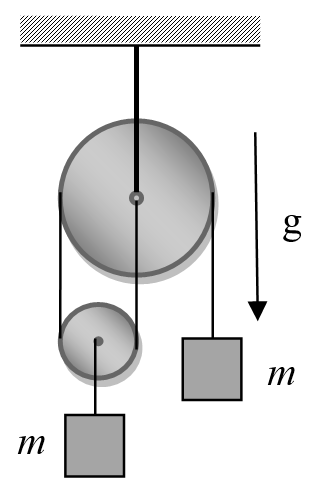
\includegraphics[width=0.2\columnwidth]{figures/03}
           \caption{A boat.}
           \label{fig:wowonaqi}
        \end{figure}

\section{კინემატიკური ბმები დინამიკის ამოცანებში}
%Черноуцан А., Кинематические связи в задачах динамики
მექანიკის ამოცანებში ხშირად გვხდება სიტუაცია, როდესაც სხეულის მოძრაობა არ არის თავისუფალი. ეს შეზღუდვა შეიძლება იყოს განპირობებული მყარი ზედაპირებით, უჭიმვადი ძაფებით, ხისტი ღეროებით და ასე შემდეგ. მარტივ შემთხვევებში ამ შეზღუდვებს ვითვალისწინებთ ავტომატურად და არც კი ვსაუბრობთ მასზე. მაგალითად სხეულის აჩქარებას პირდაპირ მივმართავთ სიბრტყის გასწვრივ (ცხადია მყარი ზედაპირის შემთხვევაში), ბუქსირზე ჩაბმული მანქანისა და მაბუქსირებელი მანქანის სიჩქარეს ვთვლით ტოლად (ვგულისხმობთ რომ მანქანები გადაბმულია უჭიმვადი ტროსით). ხანდახან კი აუცილებელია ეს შეზღუდვა აღვწეროთ სპეციალური განტოლებების საშუალებით, რომელთაც ჩვენ ვუწოდებთ \textbf{კინემატიკურ ბმას}. განვიხილოთ რამდენიმე ამოცანა.
%\begin{figure}
%\centering
%\begin{minipage}{.5\textwidth}
%  \centering
%  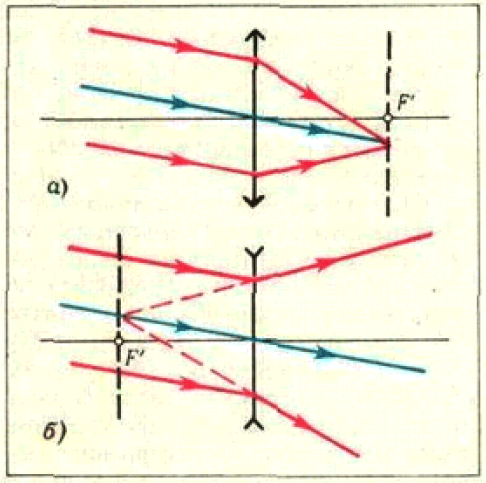
\includegraphics[width=.9\linewidth]{figures/optics_2}
%  \captionof{figure}{სხივთა სვლა თხელ ა) შემკრებ, ბ) გამბნევ ლინზაში.}
%  \label{fig:optics_1}
%\end{minipage}%
%\begin{minipage}{.5\textwidth}
%  \centering
%  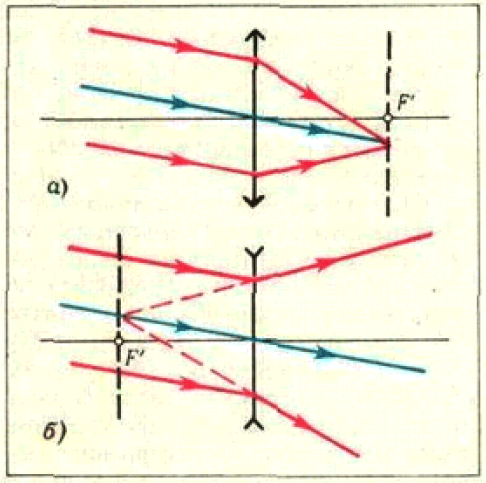
\includegraphics[width=.9\linewidth]{figures/optics_2}
%  \captionof{figure}{ლინზაზე დაცემულ პარალელურ სხივთა სვლა თხელ ა) შემკრებ, ბ) გამბნევ ლინზაში.}
%  \label{fig:optics_2}
%\end{minipage}
%\end{figure}
 
 
\section{მოძრაობა მოსახვევში}
%Асламазов Л., Движение по окружности
წრეწირზე მოძრაობისას აღწერისას წრფივი სიჩქარის მცნებასთან ერთად შემოაქვთ კუთხური სიჩქარის განმარტებაც. თუკი ნივთიერი წერტილი წრეწირზე მოძრაობისას $\Delta t$ დროში შემოწერს რკალს, რომლის კუთხური ზომაა $\Delta \phi$, მაშინ კუთხური სიჩქარეა $\omega = \frac{\Delta \phi}{\Delta t}$.

%ბენდრიკოვი 301
განსაზღვრე პლანეტის $\rho$ საშუალო სიმკვრივე, თუ ეკვატორზე დინამომეტრზე ჩამოკიდებული ტვირთი $10~\%$-ით მსუბუქია ვიდრე პოლუსზე. დღეღამის ხანგრძლივობა პლანეტაზე $t = 6$ სთ-ია.

\section{ამოცანები}
\section{მეშვიდე კლასი.}
ამოცანა ნომერი 4. ერთ ქვეყანაში გეოლოგმა იპოვა შავი მეტეორიტი
	 
\section{წრეწირზე მოძრაობა}
	 \textbf{01.} მოტოციკლეტისტი მოძრაობს ჰორიზონტალურ ზედაპირზე $v = 70$ კმ/სთ სიჩქარით, ბრუნდება $R = 100$ მ რადიუსის მოსახვევში, რა კუთხით უნდა გადაიხაროს რომ არ დაეცეს? \\
	 ამოხსნა\\
	 აქაც ხახუნის ძალაა, ძალა რომელიც აჩერებს მოტოციკლისტს, $F_{fr} = \frac{m v^2}{R}$, საყრდენის რეაქციის ძალა $N = mg$. მომენტების წესი სიმძიმის ცენტრის მიმართ მომცემს განტოლებას $F_{fr}\cdot l \sin \alpha = N l \cos \alpha$. აქ მოცემული არაა $\mu$ და მაგიტომ გვჭირდება. ეს მომენტები.
	 
	\textbf{02.} რა მაქსიმალური $v$ სიჩქარით შეიძლება იმოძრაოს მანქანამ $\alpha$ კუთხით დახრილ სიბრტყეზე თუ სიმრუდის რადიუსია $R$ და ხახუნის კოეფიციენტი ბორბლებსა და გზას შორის არის $k$.
			\begin{figure}[H]
           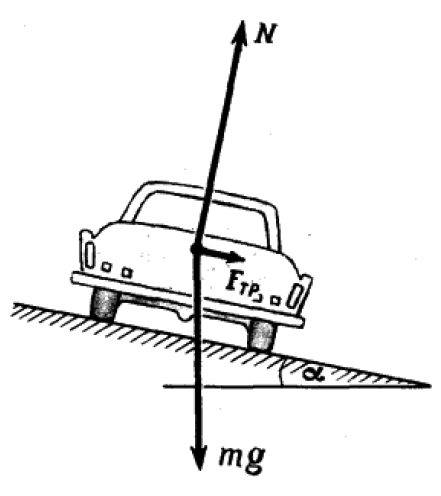
\includegraphics[width=0.2\columnwidth]{figures/02}
           \caption{A boat.}
           \label{fig:02}
        \end{figure}
        
\section{კოსმოსი}
\subsection{ნიუტონის გრავიტაციული ფორმულა}
ორი ნივთიერი წერტილი ერთმანეთს მიიზიდავს ძალით, რომელიც პირდაპირპროპორციულია მათი მასების ნამრავლისა და უკუპროპორციულია მათ შორის მანძილის კვადრატის.
	\begin{equation}
		F = G\frac{m_1 m_2}{r^2}
	\end{equation}
ანდა ჩაწერილი ვექტორული ფორმით.
	\begin{equation}
		\vec{F} = G\frac{m_1 m_2}{r^3}\vec{r}
	\end{equation}
$G = 6.67 \times 10^{-11} \dfrac{\text{ნ}\cdot\text{მ}^2}{\text{კგ}^2}$ კოეფიციენტს მსოფლიო მიზიდულობის ანუ გრავიტაციული მუდმივი ეწოდება.
ის პირველად ინგლისელმა ფიზიკოსმა ჰენრი კავენდიშმა განსაზღვრა ცდით.
\subsection{ელიფსი}%ნიკოს ნოუთები


\subsection{კეპლერის კანონები}%ნიკოს ნოუთები
\subsubsection{კეპლერის პირველი კანონი}
	პლანეტები მოძრაობს ელიფსებზე, რომელთა ერთ-ერთ ფოკუსში იმყოფება მზე.
\subsubsection{კეპლერის მეორე კანონი}
პლანეტის რადიუს-ვექტორი დროის ტოლ შუალედებში ტოლ ფართობებს მოხვეტს.
		\begin{figure}[H]
		   \centering
           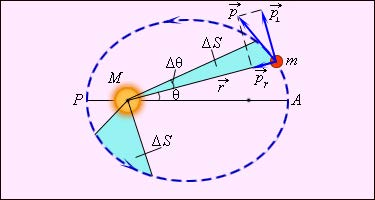
\includegraphics[width=0.5\columnwidth]{figures/kepler_2_law}
           \caption{კეპლერის მეორე კანონი - მოხვეტილი ფართობების ტოლობის კანონი.}
           \label{fig:kepler_2_law}
        \end{figure}
	
\subsubsection{კეპლერის მესამე კანონი}
	პლანეტების გარშემოვლის პერიოდების კვადრატები ისე შეეფარდება ერთმანეთს, როგორც მათი ორბიტების დიდი ნახევარღერძების კუბები.
	\begin{equation}
		\frac{T_1^2}{T_2^2} = \frac{a_1^3}{a_2^3}
	\end{equation}
	
\subsection{გრავიტაციული ურთიერთქმედების პოტენციალური ენერგია}
	$r$ მანძილით დაშორებული $m_1$ და $m_2$ მასის ნივთიერი წერტილების გრავიტაციული ურთიერთქმედების პოტენციალური ენერგიის ფორმულის მიღებას ინტეგრების ცოდნა სჭირდება. ჩვენ მოვიყვანთ შედეგს გამოყვანის გარეშე:
	\begin{equation}
		U = -G\frac{m_1 m_2}{r} + C
	\end{equation}
სადაც $C$ ნებისმიერი მუდმივაა. მისი კონკრეტული მნიშვნელობა დამოკიდებულია ნულოვანი დონის არჩევაზე. ჩვეულებრივ, ნულად თვლიან
უსასრულოდ დაშორებული სხეულების პოტენციალურ ენერგიას. ამ შემთხვევაში	$C = 0$ და $$U = -G\frac{m_1 m_2}{r}$$.
	
\subsection{კოსმოსური სიჩქარეები}
\subsubsection{პირველი კოსმოსური სიჩქარე}
პირველი კოსმოსური სიჩქარე არის ის სიჩქარე, რომელიც საჭიროა სხეულს მივანიჭოთ გასროლისას რომ არ დაეცეს უკან დედამიწაზე და გააგრძელოს მის გარშემო ბრუნვა. სხეულისთვის დავწეროთ ნიუტონის მეორე კანონი:
		\begin{equation}
			\frac{mv^2}{r_E} = G\frac{M_Em}{r_E^2}
			\label{eq:first_cosmic_speed}
		\end{equation}
სადაც $M_E$ არის დედამიწის მასა, $r_E$ არის დედამიწის რადიუსი. განვიხილავთ დედამიწასთან ახლოს მბრუნავ თანამგზავრს ამიტომაც $r_E$ არის დედამიწის რადიუსი და დედამიწის ზედაპირიდან დაშორებას არ ვითვალისწინებთ.

\ref{eq:first_cosmic_speed} განტოლებიდან მივიღებთ:
	\begin{equation}
		v = \sqrt{\frac{G M_m}{r_E}}
	\end{equation}
თუ გავითვალისწინებთ იმასაც რომ თავისუფალი ვარდნის აჩქარება $g = GM/r_E^2$ საბოლოოდ მივიღებთ:
	\begin{equation}
		v = \sqrt{g r_E} = 7.91 \times 10^3 ~ \text{მ/წმ}
	\end{equation}
	
\subsubsection{მეორე კოსმოსური სიჩქარე}
მეორე კოსმოსური სიჩქარის მინიჭებისას სხეულს შეუძლია დატოვოს დედამიწის ორბიტა, თუკი ჩავწერთ სრულ მექანიკურ ენერგიას. 
			\begin{equation}
				E = \frac{mv^2}{2} - G\frac{M_E m}{r_E}
			\end{equation}
სადაც $m$ არის სხეულის მასა, $M_E$ დედამიწის მასა, $r_E$ დედამიწის რადიუსი. 

ცხადია როდესაც დედამიწის დატოვებს მას აღარ ექნება დედამიწასთან ურთიერთქმედების პოტენციალური ენერგია, და რადგან მინიმალურ სიჩქარეს ვეძებთ აღარც კინეტიკური ენერგია ექნება ორბიტის დატოვებისას მაშინ
			\begin{equation}
				\frac{mv^2}{2} - G\frac{M_E m}{r_E} = 0
			\end{equation}
აქედან მივიღებთ:
			\begin{equation}
				v = \sqrt{\frac{2GM_E}{r_E}} = \sqrt{2 g r_E} = 11.2 \times 10^3 ~ \text{მ/წმ}
			\end{equation}

\subsubsection{მესამე კოსმოსური სიჩქარე}
მესამე კოსმოსური სიჩქარეს თუ მივანიჭებთ სხეულს დედამიწის მიმართ, ის გაექცევა მზეს.


\subsection{ამოცანები}
\textbf{01.} რა დროში დაეცემა მთვარე დედამიწას თუ ის სწრაფად გაჩერდება.\\
ამოხნსა: ამ ამოცანაში უნდა გამოვიყენოთ კეპლერის მესამე კანონი:
	\begin{equation}
		\frac{T_1^2}{T_2^2} = \frac{a_1^3}{a_2^3}
	\end{equation}
დავარდნა შეიძლება განვიხილოთ როგორც ძალიან გაწელილი ელიფსი. თუ დავუშვებთ რომ თავიდან მთვარის რადიუსი იყო $a$ ახალი რადიუსი იქნება $a/2$, მაშინ ვარდნის დრო იქნება.
	\begin{equation}
		T_1^2 = T_2^2\cdot\frac{(a/2)^3}{a^3} = T_2^2 \frac{1}{8}
	\end{equation}
სადაც $T_2$ არის ძველი მთვარის პერიოდი, მაშინ დავარდნის დრო იქნება პერიოდის ნახევარი $T_1/2$

\textbf{02.} უძრავად დამაგრებული $M$ მასის ნივთიერი წერტილის გრავიტაციულ ველში დიდი მანძილით დაშორებული წერტილიდან (ამ მანძილზე
გრავიტაციული ურთიერთქმედება შეგვიძლია უგულებელვყოთ) $v$ სიჩქარით მოძრაობს $m$ მასის ნივთიერი წერტილი, რომლის სამიზნე პარამეტრია $\rho$. იპოვეთ უმცირესი მანძილი ნივთიერ წერტილებს შორის.
		\begin{figure}[h]
		   \centering
           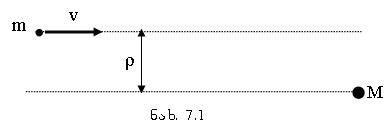
\includegraphics[width=0.5\columnwidth]{figures/fig_1}
           \caption{ამოცანა.}
           %\label{fig:boat1}
        \end{figure}
        
ამოხსნა:	იხსნება იმპულსის მუდმივობისა და ენერგიის მუდმივობით.\\
პასუხი: $$ r_{min} = \frac{1}{v^2} $$

\chapter{სითბური მოვლენები}
\section{სითბური ბალანსი}
თუ ნივთიერება დნება $+\lambda m$ გამყარება $-\lambda m$, თუ ნივთიერება ორთქლდება $+r m$ კონდესირდება $-rm$.
\section{ამოცანები.}

\chapter{ელექტრობა}

\chapter{გეომეტრიული ოპტიკა}
\section{ჩრდილი და ნახევარჩრდილი} 
თუ სხეულს დავანათებთ წერტილოვანი წყაროდან, მაშინ საგნის ჩრდილი იქნება სრული, მკვეთრად შემოხაზული საზღვარით. 
%https://en.wikipedia.org/wiki/Umbra,_penumbra_and_antumbra#Penumbra
		\begin{figure}[H]
		   \centering
           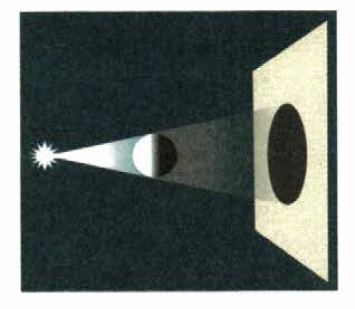
\includegraphics[width=0.3\columnwidth]{figures/shadow}
           \caption{ჩრდილი.}
           \label{fig:shadow}
           %რუსული გენდელშტაინი
        \end{figure}
        
თუკი ობიექტს ვანათებთ არაწერტილოვანი გაწელილი სინათლის წყაროთი, მაშინ ის ასევე წარმოქმნის ნახევარჩრდილს - ნაწილობრივ განათებულ ეკრანის არეს, სადაც მხოლოდ მანათობელი ობიექტის ნაწილიდან ეცემა სინათლე. ზოგიერთ შემთხვევაში შეიძლება სრული ჩრდილი საერთოდ არ გვქონდეს, და მხოლოდ იყოს ნახევარჩრდილი.
		\begin{figure}[H]
		   \centering
           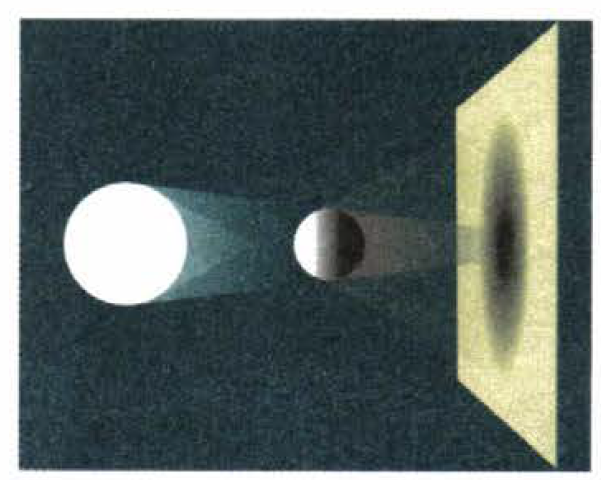
\includegraphics[width=0.3\columnwidth]{figures/penumbra}
           \caption{ნახევარჩრდილი.}
           \label{fig:penumbra}
           %რუსული გენდელშტაინი
        \end{figure}
        
ნახევარჩრდილის ზომის და გეომეტრიული ფორმის განსაზღვრა შესაძლებელია გეომეტრიული აგებით, სინათლის წრფივი გავრცელების მიხედვით.

\section{თხელი ლინზები} ლინზას ორი სფერული ზედაპირით შემოსაზღვრულ გამჭვირვალე სხეულს უწოდებენ. თუ მისი სისქე მცირეა სფერული ზედაპირების სიმრუდის რადიუსთან შედარებით, მაშინ ლინზას თხელს უწოდებენ \ref{fig:thin_lenses}.
		\begin{figure}[h]
		   \centering
           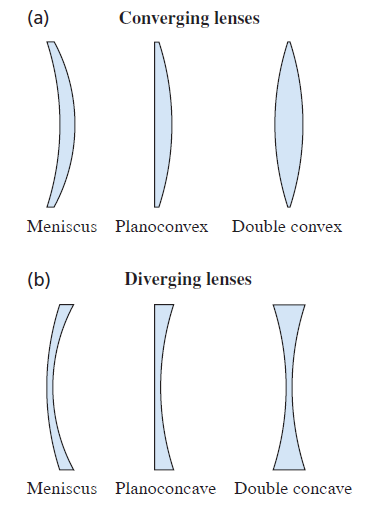
\includegraphics[width=0.4\columnwidth]{figures/thin_lenses}
           \caption{სხივთა სვლა თხელ ა) შემკრებ, ბ) გამბნევ ლინზაში.}
           \label{fig:thin_lenses}
        \end{figure}


ლინზები პრაქტიკულად ყველა ოპტიკური ხელსაწყოს შემადგენლობაში შედიან. არსებობს შემკრები და გამბნევი ლინზები. შემკრები ლინზა შუაში უფრო სქელია ვიდრე კიდეებზე, გამბნევი კი პირიქით, შუაშია უფრო თხელი.

თხელი ლინზის ფორმულა
	\begin{equation}
		\frac{1}{f} + \frac{1}{d} = \frac{1}{F}
	\end{equation}

$D$ სიდიდე ფოკუსური მანძილის შებრუნებულია და ლინზის ოპტიკურ ძალას უწოდებენ. ოპტიკური ძალის ერთეულია დიოპტრი. დიოპტრი ერთი მეტრი ფოკუსური მანძილის მქონე ლინზის ოპტიკური ძალაა:

%	\begin{tabular}{ |c|c|c| }
%		\centering
%		\hline
%		სიდიდე & ნიშანი & col3 \\
%		\hline
%		გამოსახულება & წარმოსახვითი & - \\ 
%		\hline
%	\end{tabular}

\section{გამოსახულების აგება ლინზებსა და სფერულ სარკეებში}
ლინზით ან სარკით მიღებული გამოსახულების ადგილმდებარეობის განსაზღვრა შეიძლება ორი მეთოდით - ალგებრული გამოთვლით (ლინზისა და სარკის ფორმულის გამოყენებით) ანდა გეომეტრიული აგებით.

პირველი მეთოდი თუმც არის უფრო უნივერსალური, ხშირად რთულ ოპტიკურ სისტემებში მას თავს ვერ ავარიდებთ. სამაგიეროდ მეორე მეთოდი უფრო თვალსაჩინოა. ამიტომაც ალგებრულად ამოცანის შემთხვევაშიც კი ვაკეთებთ ნახაზს, რომელიც გვეხმარება საჭირო სისტემის დაწერაში. თუ ამოცანა არ არის ზედმეტად შრომატევადი(?), აგებით ამოხსნა არის უფრო მოსახერხებელი.

თხელ ლინზებში გამოსახულების აგებისას ვსარგებლობთ სამი ძირითადი თვისებით სინათლის სხივის ნახ.ა)~\ref{fig:optics_1}.
		\begin{figure}[h]
		   \centering
           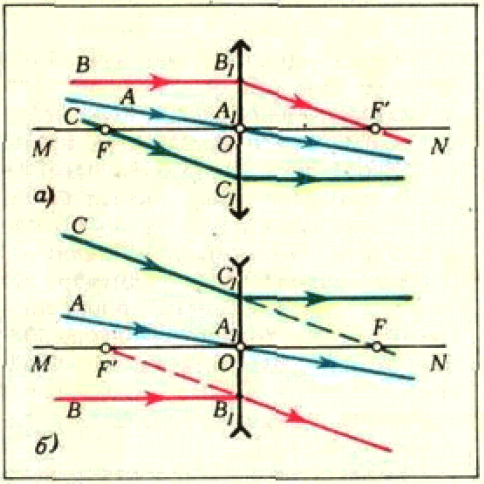
\includegraphics[width=0.5\columnwidth]{figures/optics_1}
           \caption{სხივთა სვლა თხელ ა) შემკრებ, ბ) გამბნევ ლინზაში.}
           \label{fig:optics_1}
        \end{figure}

1) სხივი $AA_1$, რომელიც გადის ლინზის ოპტიკურ ცენტრში $O$ (მეორენაირად ეძახიან დამხმარე ოპტიკურ ღერძს) არ გარდატყდება.

2) სხივი $BB_1$,რომელიც ეცემა ლინზას მთავარი ოპტიკური ღერძის პარალელურად გარდატყდება და გაივლის ლინზის უკანა $F'$ ფოკუსსი.

3) სხივი $CC_1$, რომელიც გადის წინა ფოკუსში $F$, ლინზაში გარდატეხის მერე გამოდის მთავარი ოპტიკური ღერძის პარალელურად.

უკანა ფოკუსი $F'$ ეწოდება წერტილს რომელშიც იკრიბებიან გარდატეხის შემდგომ ოპტიკური ღერძის პარალელურად,ლინზაზე დაცემული სხივები. წინა $F$ და უკანა $F'$ ფოკუსები განლაგებულები არიან თხელი ლინზის მიმართ სიმეტრიულად. $F$ გადის უკანა ფოკალური სიბრტზე, $F'$-ში გადის უკანა ფოკალური სიბრტყე.

ხანდახან ასევე გვეხმარება შემდეგი წესებიც:
1) სხივები, რომლებიც ლინზას ეცემიან პარალელურ ნაკადად, გარდატეხის შემდეგ იკრიბებიან უკანა ფოკალურ სიბრტყეში~\ref{fig:optics_2}.

2) სხივები რომლებიც გამოდიან ლინზიდან პარალელურ ნაკადად, ლინზაზე დაცემამდნენ გადაიკვეთნენ წინა ფოკალურ სიბრტყეში~\ref{fig:optics_3}. 

		\begin{figure}[h]
		   \centering
           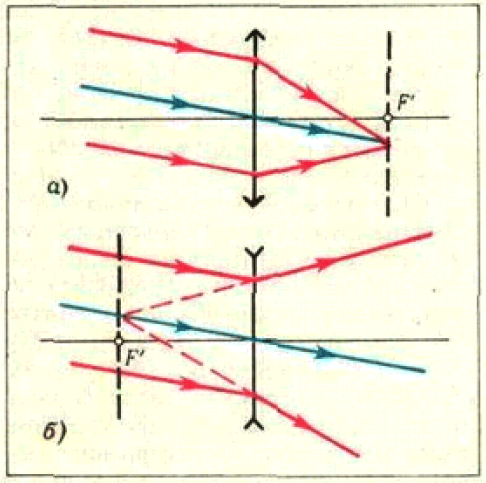
\includegraphics[width=0.5\columnwidth]{figures/optics_2}
           \caption{ლინზაზე დაცემულ პარალელურ სხივთა სვლა თხელ ა) შემკრებ, ბ) გამბნევ ლინზაში.}
           \label{fig:optics_2}
        \end{figure}

		\begin{figure}[h]
		   \centering
           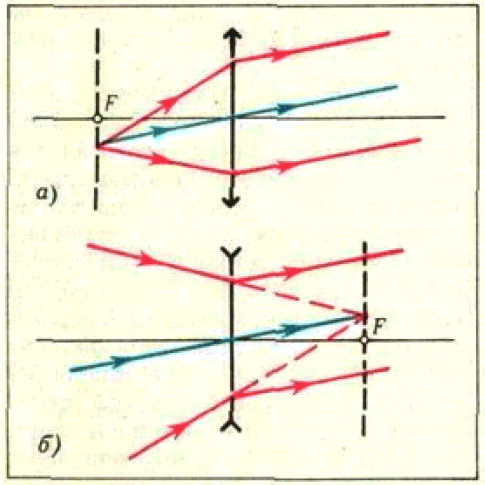
\includegraphics[width=0.5\columnwidth]{figures/optics_3}
           \caption{ლინზიდან გამოსული პარალელურ სხივთა "უკუსვლა" თხელ ა) შემკრებ, ბ) გამბნევ ლინზაში.}
           \label{fig:optics_3}
        \end{figure}

\section{სფერული სარკე}


\section{ამოცანები.}

\textbf{..} 
ორ ბრტყელ სარკეს შორის კუთხე არის $\alpha$. იპოვეთ სარკეებს შორის მოთავსებული მნათი წერტილის რამდენი გამოსახულება მიიღება ასეთ სარკეში.

\textbf{01.}
%იროდოვი 216
როგორია დაცემის კუთხე, თუ წყლის ზედაპირიდან არეკვლილი სხივი გარდატეხილი სხივის პერპენდიკულარულია.

\textbf{02.}
%იროდოვი 218
სინათლის სხივი ეცემა $d = 0.6$ სმ სისქის ბრტყელი პარალელური მინის ფირფიტას.დაცემის კუთხე $60 \degree$-ია. იპოვეთ ამ ფირფიტაში გასული სხივის წანაცვლების სიდიდე.
\end{document}